\documentclass[border=10pt]{standalone}
\usepackage{tikz}
\usetikzlibrary{shapes, arrows, positioning}

\begin{document}
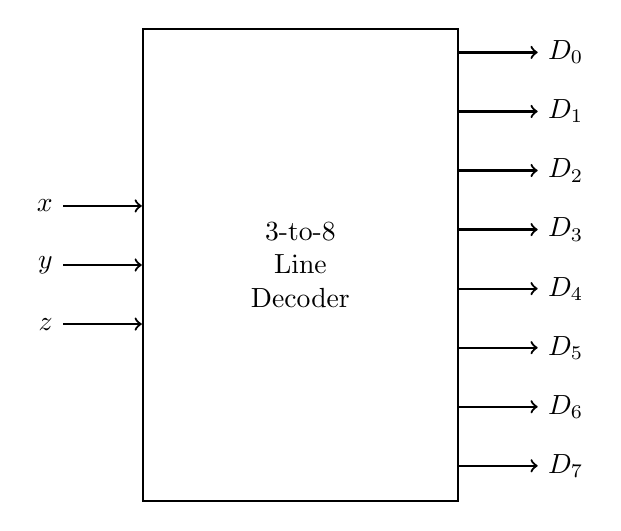
\begin{tikzpicture}[
    thick,
    node distance=1.5cm,
    block/.style={draw, rectangle, minimum height=6cm, minimum width=4cm, align=center, fill=white}
]

    % Main Block
    \node[block] (decoder) {3-to-8\\Line\\Decoder};

    % Inputs
    \foreach \i/\label in {1/x, 2/y, 3/z} {
        \draw[<-] (decoder.west) ++(0, 1.5 - \i*0.75) coordinate (in\i) -- ++(-1,0) node[left] {$\label$};
        \node at (in\i) [right, xshift=2mm] {}; % Internal label if needed
    }

    % Outputs
    \foreach \i/\label in {0/D_0, 1/D_1, 2/D_2, 3/D_3, 4/D_4, 5/D_5, 6/D_6, 7/D_7} {
        \draw[->] (decoder.east) ++(0, 3.2 - \i*0.75 - 0.5) coordinate (out\i) -- ++(1,0) node[right] {$\label$};
    }

\end{tikzpicture}
\end{document}
